% !TeX root = ../../Lezione1.tex
\section{Memory (HTML)}

\begin{frame}\transfade
  \begin{exercise}\centering
    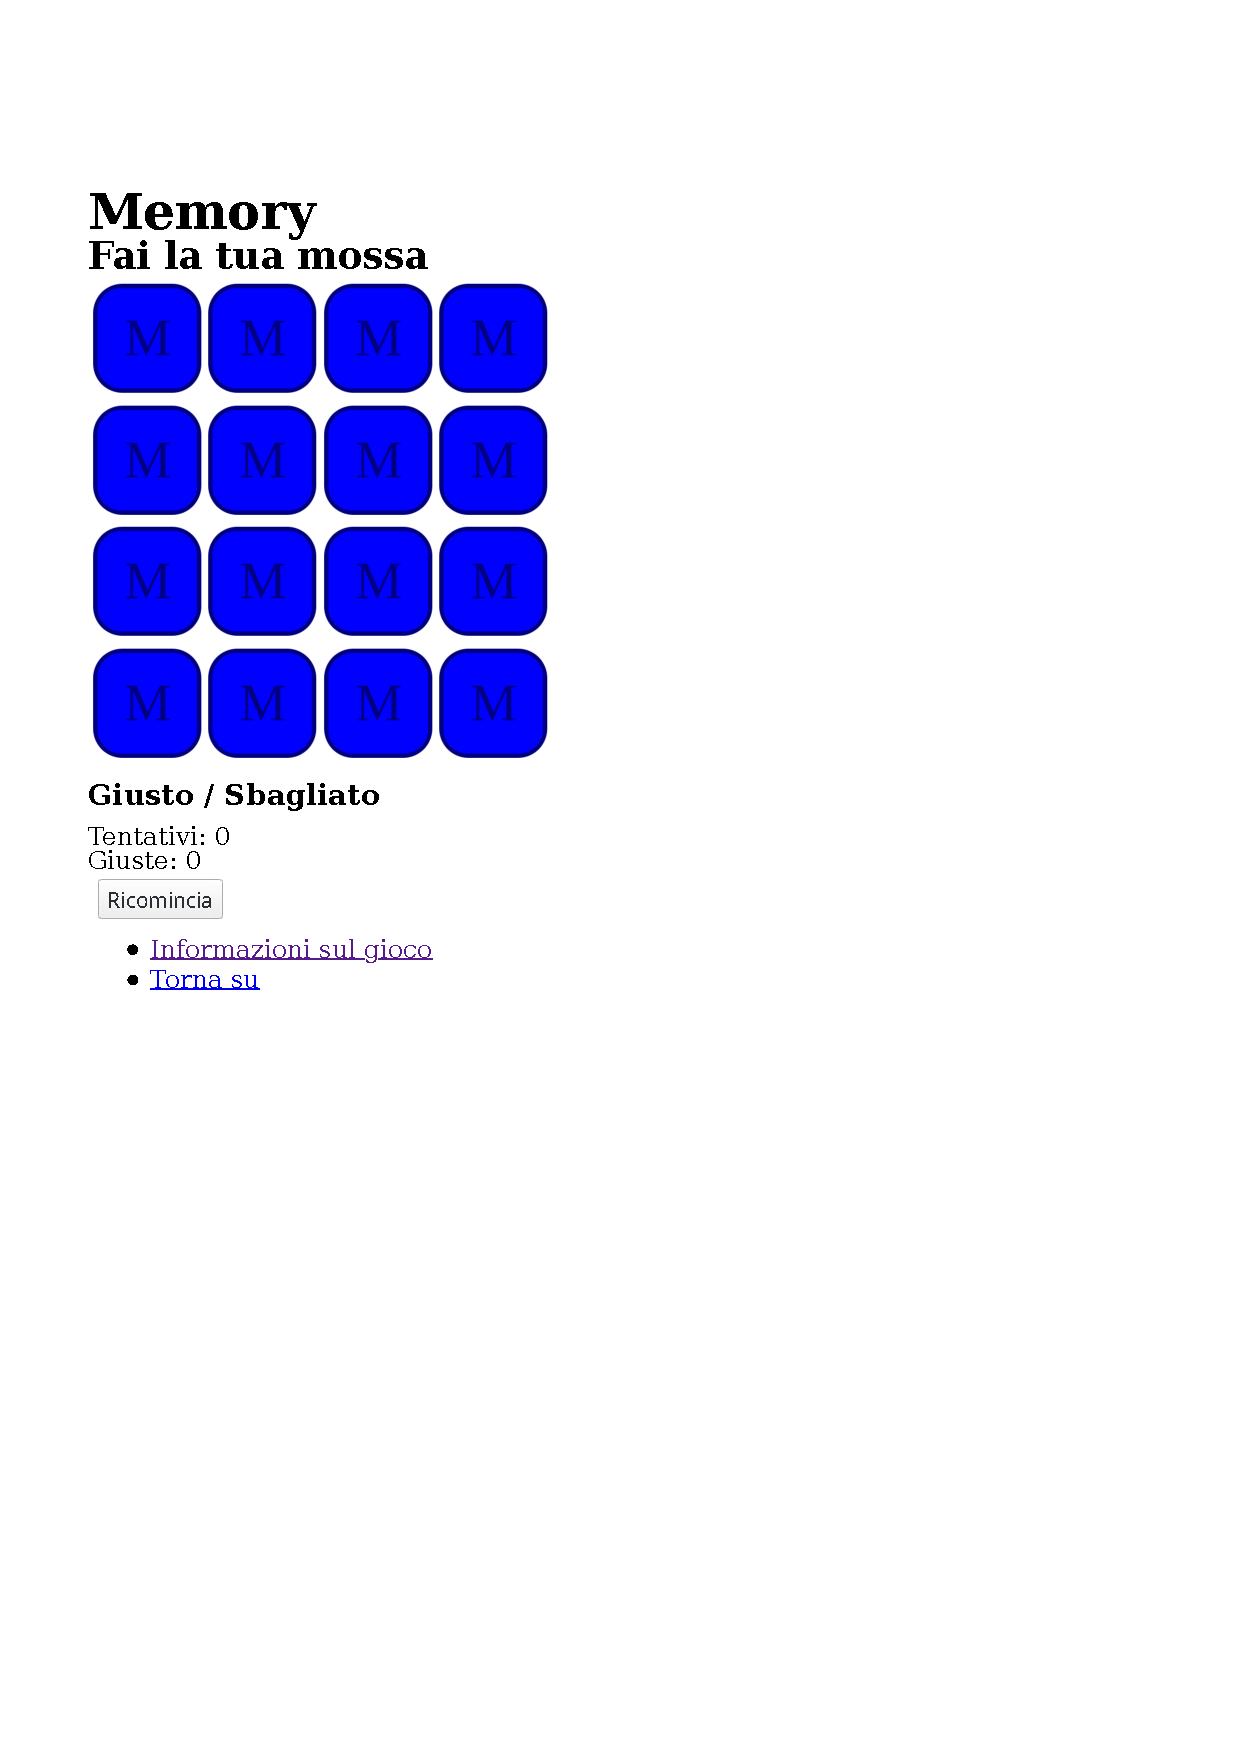
\includegraphics[height=.85\textheight]{memory/html/memory.pdf}
  \end{exercise}
\end{frame}

\begin{frame}[fragile]\transfade
  \begin{sol}\centering
    \begin{minted}{html}
<button> Ricomincia </button>
    \end{minted}
  \end{sol}
\end{frame}

\begin{frame}[fragile]\transfade
  \begin{sol}\centering
    \inputminted[lastline=17]{html}{memory/html/memory.html}
    continua\dots
  \end{sol}
\end{frame}
\begin{frame}[fragile]\transfade
  \begin{sol}\centering
    \inputminted[firstline=18, lastline=43, fontsize=\tiny]{html}{memory/html/memory.html}
    continua\dots
  \end{sol}
\end{frame}
\begin{frame}[fragile]\transfade
  \begin{sol}\centering
    \inputminted[firstline=45, breaklines]{html}{memory/html/memory.html}
  \end{sol}
\end{frame}